\begin{figure}[htbp]
\centering
\shorthandoff{<>}
\begin{tikzpicture}[x=1.4cm,y=34cm,font=\normalsize,>=latex]
  \fill[green!9] (6.0025,0) rectangle (10,0.02);
  \draw[->,black!65] (0,0) -- (10.5,0) node[right] {$n$};
  \draw[->,black!65] (0,0) -- (0,0.105) node[above,align=center] {Semiancho\\máximo};
  \foreach \y/\lab in {0.02/{0.02},0.04/{0.04},0.06/{0.06},0.08/{0.08},0.10/{0.10}}{
    \draw[black!12] (0,\y) -- (10,\y);
    \node[left] at (0,\y) {$\lab$};
  }
  \draw[blue!75!black,very thick,domain=0.25:10,samples=150]
    plot (\x,{0.049/sqrt(\x)});
  \draw[dashed,orange!85!black,thick] (0,0.02) -- (10,0.02);
  \draw[dashed,orange!85!black,thick] (6.0025,0) -- (6.0025,0.02);
  \fill[orange!85!black] (6.0025,0.02) circle (2.4pt);
  \node[above left,align=left,orange!85!black] at (6.0,0.024)
    {$n_{\min}=2401$\\$E=0.02$};
  \node[blue!75!black,anchor=west,align=left] at (1.0,0.083)
    {$E_{\max}(n)=1.96\sqrt{\dfrac{0.25}{n}}$};
  \node[align=center,green!35!black] at (8.0,0.054)
    {Se garantiza\\ancho $\le0.04$};
  \foreach \x/\lab in {0/0,2/800,4/1600,6/2400,8/3200,10/4000}{
    \draw (\x,0)--(\x,-0.0015) node[below] {$\lab$};
  }
\end{tikzpicture}
\shorthandon{<>}
\caption{Semiancho conservador de un intervalo normal aproximado del 95\% cuando se desconoce la proporción. Se usa $p=0.5$, que maximiza $p(1-p)$ y por tanto el tamaño de muestra requerido. El ancho total es el doble del semiancho representado.}
\label{fig:tamano-muestra}
\end{figure}